Dans ce chapitre, l'objectif est d'effectuer une analyse approfondie de chaque composant du système afin de déterminer leurs caractéristiques et spécifications respectives.
Cette analyse permettra ensuite de sélectionner les composants à utiliser pour la réalisation du système.

\section{Bus de communication}

Dans le cadre de ce projet, le bus de communication envisagé est l'I2C.
Cependant, il est pertinent de comparer ce bus avec d'autres protocoles de communication pour déterminer le plus adapté.
Il existe une variété de bus de communication disponibles.
Pour ce projet, il est nécessaire de choisir un protocole simple et compact, en accord avec les exigences des systèmes embarqués.

Dans ce projet, le nombre maximal de périphériques n'est pas clairement défini.
Il est donc important de sélectionner un protocole offrant une capacité maximale en termes de nombre de périphériques, afin de ne pas être limité par cette contrainte à l'avenir.

La vitesse de transfert des données doit être suffisante pour permettre la transmission des informations des capteurs et des actionneurs.
Cependant, la vitesse de transfert des données n'est pas un critère critique pour ce projet.

Enfin, le nombre de fils de communication est un paramètre important à prendre en compte.
En effet, il est nécessaire de limiter au maximum le nombre de fils de communication afin de prévenir la complexité du câblage et de réduire l'encombrement.

Afin de faciliter cette comparaison, un tableau comparatif des différents bus de communication pertinents pour ce projet est présenté ci-dessous.

\begin{table}[H]
    \begin{center}
        \caption{Bus de communication \label{tab:buscommunication}}
        \begin{tabular}{c|c|c|c}
            Nom & \begin{tabular}[c]{@{}c@{}}Nombre maximal\\ de périphériques\end{tabular} & Vitesse standard & Fils de communication \\ \hline
            I2C & 127                                                                       & 0.1 Mbit/s       & 2                     \\
            CAN & Non défini                                                                & 1 Mbit/s         & 2                     \\
            LIN & 16                                                                        & 0.02 Mbit/s      & 1                     \\
            SPI & Non défini                                                                & 10 Mbit/s        & 4
        \end{tabular}
    \end{center}
\end{table}

La vitesse spécifiée représente la vitesse standard du bus, mais dans certains cas, la vitesse peut être supérieure avec une autre configuration.

\subsection{LIN}

Le bus LIN est le bus de communication le plus lent et a un nombre réduit de périphériques par rapport aux autres.
Il est donc écarté.

\subsection{SPI}

Le bus SPI a une particularité, le nombre de fils de communication dépend du nombre de périphériques connectés.
En effet, il possède quatre signaux logiques : \texttt{SCLK} (Serial Clock) qui est l'horloge du bus, \texttt{MOSI} (Master Output Slave Input) qui est la ligne de données du maître vers l'esclave, \texttt{MISO} (Master Input Slave Output) qui est la ligne de données de l'esclave vers le maître et \texttt{SS} (Slave Select) qui est la ligne de sélection de l'esclave.
Le nombre de fils de communication est donc égal à trois plus le nombre de périphériques esclaves.
Ce bus ne convient pas à ce projet, car il n'est pas simple d'ajouter ou de retirer des périphériques.

\subsection{CAN}

Le bus CAN possède une vitesse intéressante par rapport aux autres bus de communication. Cependant, lorsqu'un composant fonctionne avec CAN, il utilise CANOpen. CANOpen est complexe à mettre en place. De plus la majorité des microcontrôleurs qui possède un contrôleur CAN doivent être connecté à un transceiver CAN qui est un autre composant. Ce bus n'est donc pas adapté à ce projet.

\subsection{I2C}

Le bus I2C est vraiment adapté pour notre projet, car il ne présente pas de défauts majeurs par rapport à d'autres bus de communication.
De plus, la plupart des composants I2C disponibles actuellement sur le marché prennent en charge le "fast mode" qui permet une vitesse de transfert allant jusqu'à 0.4 Mbit/s.

Une autre caractéristique intéressante de l'I2C est son mode multimaître, qui peut être utile dans certaines situations.
En résumé, l'I2C répond parfaitement à nos exigences pour ce projet, offrant une vitesse de transfert suffisante et la flexibilité nécessaire.

\section{Microcontrôleur}

Dans cette section, une analyse des microcontrôleurs disponibles sur le marché sera réalisée dans le but de déterminer celui qui convient le mieux à ce projet.
De plus, une évaluation des langages de programmation les plus couramment utilisés pour les microcontrôleurs sera effectuée.
Il sera également nécessaire de choisir le boîtier le plus approprié pour le microcontrôleur sélectionné.
Après ces analyses, d'autres critères devront être définis.
Par exemple, il est spécifié dans le cahier des charges que le microcontrôleur doit être équipé d'un ARM Cortex.
De plus, il est essentiel d'avoir les périphériques couramment utilisés tels que UART, SPI, I2C, GPIO, ADC et PWM.
Ces critères devront être pris en compte lors du choix final du microcontrôleur.

\subsection{Fabricants}

Dans le domaine des microcontrôleurs, il existe plusieurs fabricants présents sur le marché.
Cependant, il est pertinent de se concentrer sur les fabricants qui détiennent une part de marché significative.
En se limitant à ces fabricants, on s'assure d'avoir accès à une documentation complète et à un approvisionnement adéquat en termes de disponibilité des composants.
Les données de \href{https://www.statista.com/statistics/1327509/top-mcu-suppliers-worldwide/}{Statista.com} fournissent un aperçu des parts de marché des fabricants de microcontrôleurs en 2021.
Voici un graphique présentant ces données.

\begin{figure}[H]
    \centering
    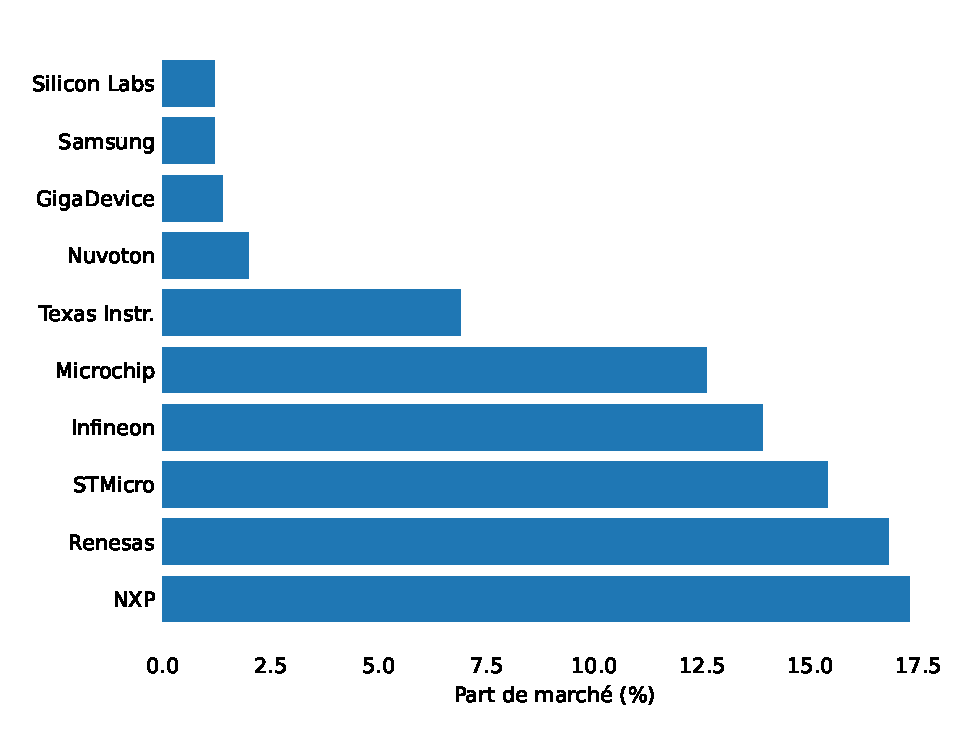
\includegraphics[width=12cm]{./assets/figures/topmcu.py.eps}
    \caption{Part de marché des fabriquants de microcontrôleurs en 2021 }
    \label{fig:topmcu}
\end{figure}

L'analyse des données révèle que NXP, Renesas, STMicro, Infineon, Microchip et Texas Instruments sont les principaux fabricants de microcontrôleurs sur le marché en 2021.
Il est donc judicieux de considérer ces fabricants en priorité lors du processus de sélection du microcontrôleur.
Chacun des fabricants mentionnés ci-dessus propose des microcontrôleurs basés sur l'architecture ARM Cortex.

\subsection{Langages de programmation}

Différents langages de programmation sont utilisés pour programmer des microcontrôleurs, mais certains sont plus répandus que d'autres.
Le langage de programmation C est largement utilisé et constitue le choix prédominant lorsqu'il s'agit de trouver du code pour les microcontrôleurs.
Dans certains cas, l'assembleur est également utilisé, notamment pour des applications spécifiques.
On trouve également des projets qui utilisent le C++, le Rust et le Python, bien que leur utilisation soit moins répandue.
La première option courante consiste donc à utiliser le langage C.
Cependant, il est intéressant d'explorer les autres langages de programmation, en particulier le C++, afin de déterminer leur pertinence pour ce projet.

Le choix du langage de programmation dépendra des fonctionnalités et des possibilités offertes par le \textit{\gls{framework}} de développement sélectionné.

\subsection{Boitiers}

Les microcontrôleurs sont disponibles dans différentes tailles de boîtiers, chacun présentant ses avantages et ses inconvénients.
Dans le cadre de ce projet, il est essentiel de choisir un boîtier compact et facile à souder.
La taille réduite du boîtier est importante, car elle permet de minimiser l'empreinte du circuit imprimé, ce qui répond aux exigences de compacité des systèmes embarqués du projet.
La facilité de soudure est également un critère important, car elle permet de réduire les coûts de production et facilite la maintenance en permettant le remplacement facile des composants défectueux.
Ainsi, la sélection du boîtier approprié contribue à la performance et à la durabilité du projet.

Le boîtier BGA offre un excellent rapport taille/nombre de broches.
Cependant, il est difficile à souder sans équipement spécifique, il est donc exclu pour ce projet.

\begin{figure}[H]
    \centering
    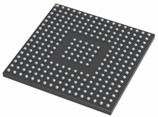
\includegraphics[scale=0.4]{./assets/figures/bga.jpg}
    \caption{\cite{bga} Boitier BGA}
\end{figure}

Le boîtier SO/SSOP est facile à souder, mais il présente une limitation en termes de nombre de broches et occupe beaucoup d'espace sur le circuit imprimé pour seulement deux rangées de broches.
Il est donc écarté.

\begin{figure}[H]
    \centering
    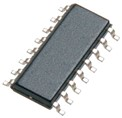
\includegraphics[scale=0.45]{./assets/figures/so_ssop.jpg}
    \caption{\cite{so_ssop} Boitier SO/SSOP}
\end{figure}

Le boîtier TQFP/LQFP est facile à souder, offre un plus grand nombre de broches que le boîtier SO/SSOP et occupe moins d'espace sur le circuit imprimé.
Il est donc intéressant pour ce projet.

\begin{figure}[H]
    \centering
    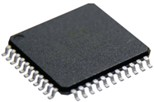
\includegraphics[scale=0.4]{./assets/figures/tqfp_lqfp.jpg}
    \caption{\cite{tqfp_lqfp} Boitier TQFP/LQFP}
\end{figure}

Enfin, le boîtier QFN est facile à souder pour quelqu'un d'expérimenté et offre un plus grand nombre de broches par rapport à sa taille.
Il occupe donc très peu d'espace sur le circuit imprimé.
Il est donc plus intéressant que le boîtier TQFP/LQFP, en tenant compte de la taille qui est un critère important pour ce projet.

\begin{figure}[H]
    \centering
    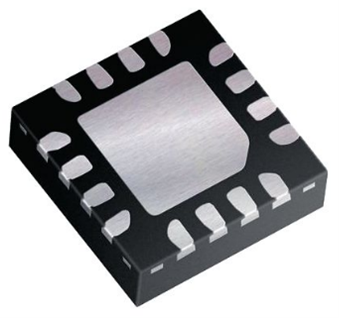
\includegraphics[scale=0.5]{./assets/figures/qfn.png}
    \caption{\cite{qfn} Boitier QFN}
\end{figure}

Ainsi, après évaluation, les boîtiers privilégiés pour ce projet sont le boîtier QFN en raison de sa compacité et de son nombre de broches plus élevé, et le boîtier TQFP/LQFP en raison de sa facilité de soudure et de son encombrement réduit par rapport au boîtier SO/SSOP.

\subsection{Choix}

Pour assurer la durabilité de ce projet, il est crucial de choisir un microcontrôleur largement utilisé, afin de pouvoir le remplacer par un modèle similaire de la même famille si celui-ci venait à être discontinué.

En Suisse, les principaux acteurs dans le domaine des sites marchands d'achat sont Digikey et Mouser.
Ces sites proposent généralement des produits similaires, avec des différences principalement liées à leur stock.
Cependant, Digikey offre un système de filtres qui permet de sélectionner les périphériques souhaités sur le microcontrôleur, ce qui est essentiel pour ce projet.
Les recherches seront donc effectuées sur Digikey.

Il convient d'appliquer les filtres suivants :

\begin{itemize}
    \item Processeur c\oe{}ur: ARM Cortex-M*
    \item En stock: Oui
    \item Connectivité: I2C, UART, SPI
    \item Périphériques: PWM
    \item Boîtier: *QFN
    \item Boîtier fournisseur: Inférieur ou égal à (4x4)
\end{itemize}

Le choix d'un c\oe{}ur ARM Cortex-M assure une architecture ARM solide, idéale pour les systèmes embarqués.
En ce qui concerne la taille du boîtier, une dimension égale ou inférieure à 4x4mm garantit la compacité du microcontrôleur.

Cependant, il y a un critère qui ne peut pas être pris en compte lors de l'application des filtres, c'est la définition du nombre de bus I2C.
En effet, il est nécessaire d'avoir deux bus de données I2C.
Un qui fera partie de l'écosystème, et un autre qui permet, si nécessaire, de piloter un périphérique I2C.
Il est donc essentiel de vérifier dans la fiche technique du microcontrôleur s'il dispose bien de deux bus I2C.

Environ 80 résultats correspondent aux critères définis.
En analysant ces résultats, il est remarqué qu'il y a une présence significative de microcontrôleurs de la famille STM32.
Cette famille est étendue, ce qui en fait un choix privilégié.
Après avoir examiné les datasheets, deux microcontrôleurs répondent aux exigences du projet : le STM32G031G6U6 et le STM32G071GBU6.
La principale différence entre les deux réside dans la quantité de mémoire flash et de RAM.
Dans ce projet, l'objectif est d'utiliser un chargeur de démarrage et un micrologiciel.
Par conséquent, il est préférable de choisir le STM32G071GBU6 qui offre une plus grande capacité de mémoire flash et de RAM.
Cela évitera de rencontrer des problèmes de mémoire lorsque des fonctionnalités supplémentaires seront ajoutées ultérieurement dans le projet.

\section{\gls{framework}s}

Pour assurer un fonctionnement simple, une maintenance aisée et une portabilité du code, l'utilisation d'un \textit{\gls{framework}} de développement est intéressante.
Celui-ci fait le lien entre un code plus abstrait et un code spécifique au microcontrôleur.
Il est important de pouvoir accéder aux fonctionnalités de bas niveau du microcontrôleur lorsque celles-ci ne sont pas réalisées de manière plus abstraite dans le \textit{\gls{framework}}.
Ainsi, il doit faciliter le développement de fonctionnalités spécifiques et disposer d'une documentation complète.
Il doit également être maintenu et utilisé par une communauté active, ce qui permet de trouver des solutions aux problèmes plus facilement.
De plus, le \textit{\gls{framework}} doit être compatible avec le microcontrôleur STM32 choisi.
Trois \textit{\gls{framework}s} potentiels répondent à ces critères, il s'agit de Mbed, Arduino et STM32Cube.
Il convient d'analyser et de comparer ces \textit{\gls{framework}s} pour déterminer lequel est le plus adapté à ce projet.

\subsection{Arduino}

Le \textit{\gls{framework}} Arduino est largement adopté par les amateurs d'électronique pour leurs projets personnels, mais il est moins couramment utilisé dans le milieu professionnel.
Bien qu'il permette une implémentation rapide des fonctionnalités, il peut manquer d'optimisation par rapport à une plateforme dédiée.
La communauté qui entoure Arduino est vaste, mais elle est principalement constituée d'amateurs.
La documentation disponible peut être moins claire, avec une prédominance de forums et de tutoriels orientés vers des projets personnels.
De plus, il n'existe pas de documentation officielle exhaustive pour chaque fonctionnalité avec des exemples spécifiques.

Une particularité d'Arduino réside dans le fait qu'il n'y a pas de licence open source unique pour ses bibliothèques.
Chaque bibliothèque peut avoir sa propre licence.
Cela peut poser des problèmes si une bibliothèque utilise la licence publique générale GNU (GPL).
Cette licence exige que le code source du projet soit disponible pour tous.
Cette situation peut être contraignante si l'on souhaite utiliser l'écosystème Arduino à des fins commerciales tout en maintenant le code source confidentiel.

\subsection{STM32Cube}

Le \textit{\gls{framework}} STM32Cube est développé par STMicroelectronics, le fabricant du microcontrôleur STM32, et il est intégré à l'IDE STM32CubeIDE.
Il offre une compatibilité optimale avec les microcontrôleurs STM32, permettant de tirer pleinement parti de leurs fonctionnalités.
Il offre une interface conviviale pour configurer les broches du microcontrôleur en fonction des fonctionnalités souhaitées.
Cependant, il peut être assez verbeux, ce qui signifie que l'utilisateur doit écrire son code dans des zones spécifiques et délimitées par des commentaires.
Cela peut rendre le code plus complexe à comprendre au premier abord, car il mélange les aspects bas niveau du microcontrôleur avec des fonctionnalités de haut niveau.

Lors de la recherche d'informations sur l'implémentation de fonctionnalités spécifiques, il peut être difficile de trouver une documentation officielle.
Cependant, les forums sont souvent une source précieuse d'informations, avec souvent des réponses fournies par des professionnels expérimentés.

\subsection{Mbed}

Mbed est un \textit{\gls{framework}} développé en collaboration par ARM et ses partenaires technologiques, spécialement conçus pour les microcontrôleurs ARM Cortex-M 32 bits.
Il offre une documentation officielle très complète, qui se classe souvent en tête des résultats de recherche lorsqu'il s'agit d'implémenter des fonctionnalités spécifiques.
Les forums Mbed sont également une ressource précieuse, avec une présence notable de professionnels expérimentés.

Ce qui est particulièrement avantageux avec Mbed, c'est sa simplicité pour mettre en place une communication complète.
La documentation officielle fournit de nombreux exemples pour la plupart des fonctionnalités, facilitant ainsi le développement.

En termes de licence, Mbed est open source, la plupart de ses composants étant sous licence BSD-3-Clause ou MIT.
Cela signifie que les utilisateurs ont la liberté d'utiliser, de modifier, de fusionner, de publier, de distribuer, de vendre et de sous-licencier le logiciel.
La seule condition est d'inclure la notice de licence et les droits d'auteur dans toutes les copies, ce qui offre une grande flexibilité pour les utilisations futures du projet, sans limiter la créativité.

\subsection{Choix}

Suite à l'analyse des trois \textit{\gls{framework}s}, Mbed est choisi comme le plus approprié pour ce projet.
Il répond de manière optimale aux critères définis.
Mbed dispose d'une documentation complète, abondamment illustrée d'exemples concrets.
Une communauté dynamique, principalement composée de professionnels expérimentés, anime les forums associés.
Le \textit{\gls{framework}} offre également un accès aux fonctionnalités de bas niveau du microcontrôleur, si besoin.
Par ailleurs, Mbed est un projet open source, accompagné d'une licence qui permet une grande flexibilité pour les futures utilisations du projet.

\section{Interface POSIX}

L'interface POSIX est employée pour interagir avec les éléments du bus, favorisant ainsi une communication efficace avec les divers composants I2C et permettant d'exploiter pleinement les fonctionnalités développées dans ce projet.
Cette interface inclut la détection des périphériques connectés au bus, la récupération des informations détaillées sur ces périphériques et la mise à jour du micrologiciel.
Dans un souci de portabilité, l'interface sera implémentée en Python, un langage largement utilisé dans le domaine de l'embarqué, offrant une rapidité de développement des applications et une compatibilité avec de nombreux systèmes d'exploitation.

\subsection{Découverte des périphériques}

Dans Linux, il existe un outil appelé \texttt{i2cdetect} qui permet de détecter tous les périphériques connectés sur le bus I2C.
Cet outil est issu du package \texttt{i2ctools}.
Cependant, il y a une subtilité à prendre en compte.
Par défaut, le programme effectue une lecture ou une écriture en fonction de l'adresse détectée.
Cette particularité est due au fait que certains microcontrôleurs, tels que les microcontrôleurs Atmel AT24RF08, se corrompent lorsqu'une écriture est effectuée.
À l'inverse, certains microcontrôleurs, notamment les microcontrôleurs d'horloge, ne répondent pas à une lecture, car ils sont en mode écriture seule.
Pour éviter ce problème, l'outil \texttt{i2cdetect} effectue des lectures ou des écritures en fonction de plages d'adresses connues correspondant aux composants problématiques.
Dans le cas de ce projet, il n'y a pas de composants posant problème, ce qui permet d'uniformiser le comportement en n'effectuant que des lectures.
Cela peut être réalisé en utilisant l'option \texttt{-r} de l'outil.

Dans le cadre de ce projet, il peut être intéressant de mettre en place une détection supplémentaire permettant de détecter uniquement les périphériques compatibles avec le projet.
À cet effet, un script Python a été développé.
Ce script permet de détecter les périphériques de l'écosystème en se basant sur une réponse prédéfinie.
Cela permet à l'utilisateur de distinguer rapidement et efficacement les périphériques compatibles avec le projet des autres périphériques présents sur le bus I2C.

Lors de la détection des périphériques, plusieurs informations peuvent être affichées.
Cela comprend notamment l'adresse, la version du micrologiciel, le type de périphérique, le groupe de périphérique, le nom et l'identifiant unique.

\subsubsection{Adresse}

L'adresse I2C d'un périphérique est intéressante à connaître, car elle permet d'utiliser le périphérique dans un autre contexte que celui de l'écosystème développé dans ce projet.

\subsubsection{Version du micrologiciel}

La version du micrologiciel présente sur le périphérique est également importante à connaître, car elle permet de comparer facilement les versions et de déterminer quels périphériques nécessitent une mise à jour éventuelle.

\subsubsection{Type de périphérique}

Le type de périphérique est utile pour faciliter la mise à jour du micrologiciel sur plusieurs périphériques simultanément.
Lorsqu'un code évolue pour un certain type de périphérique, il est avantageux de pouvoir mettre à jour tous les périphériques de ce type en même temps.

\subsubsection{Groupe de périphérique}

Le groupe de périphérique est un sous-filtre du type de périphérique, permettant de différencier des périphériques d'un même type.
Cela est particulièrement utile lorsque différents groupes de périphériques du même type présentent des fonctionnalités différentes, afin de ne mettre à jour que les périphériques concernés par les changements de firmware.

\subsubsection{Nom}

Le nom du périphérique est intéressant pour l'utilisateur. En effet, il permet de différencier les périphériques entre eux. Cela permet de faire un lien plus rapide entre l'affichage et le périphérique physique.

\subsubsection{Identifiant unique}

L'identifiant unique est un identifiant distinct attribué à chaque périphérique.
Il permet de différencier de manière unique les périphériques les uns des autres.
Cet identifiant est prédéfini par le fabricant et ne peut être modifié.
Grâce à ce champ, il est possible à tout moment de distinguer les périphériques entre eux de manière univoque.

\subsection{Mise à jour du micrologiciel}

La mise à jour du micrologiciel est une fonctionnalité clé de l'interface POSIX.
Elle permet de mettre à jour facilement et efficacement le micrologiciel des périphériques concernés, sans avoir besoin de connecter un câble spécifique pour la programmation de la carte.
En utilisant la commande de mise à jour appropriée, le programme est en mesure de téléverser le nouveau micrologiciel sur le périphérique cible.
Une fois la mise à jour terminée avec succès, le périphérique redémarre avec le nouveau micrologiciel.

La mise à jour du micrologiciel peut être réalisée en utilisant l'adresse I2C du périphérique, le type de périphérique ou le groupe de périphériques.
Cette flexibilité permet de mettre à jour un ou plusieurs périphériques simultanément en exécutant une seule commande.

\section{Auto-adressage}

Sur un bus I2C, chaque périphérique doit avoir une adresse unique.
Cependant, les périphériques utilisent la même méthode de génération, il est alors nécessaire de générer des adresses différentes tout en utilisant le même algorithme.
Il est donc important de trouver une méthode pour générer une adresse unique pour chaque périphérique.

\subsection{Méthode de génération}

La méthode de génération d'adresse repose sur l'utilisation de l'identifiant unique de chaque périphérique.
Grâce à cet identifiant, il est possible de générer une adresse différente pour chaque périphérique tout en utilisant le même algorithme.
Il est cependant essentiel de garantir l'unicité des adresses générées à partir de cet identifiant.

Dans un premier temps, il est nécessaire de définir une plage d'adresses dans laquelle les périphériques peuvent être adressés.
Pour ce projet, la plage d'adresses est définie entre 0x10 et 0x6F.
Cette plage permet d'adresser jusqu'à 96 périphériques différents et évite les adresses réservées situées aux extrémités de la plage tout en ayant de la marge.

En utilisant cette formule spécifique, il est possible de calculer une adresse comprise entre 0x10 et 0x6F pour chaque périphérique, en fonction de son identifiant unique.

\begin{center}
    adresse = (identifiant unique \% 96) + 0x10
\end{center}

Cependant, il est possible que deux périphériques obtiennent la même adresse malgré des identifiants uniques différents.
Afin de résoudre ce problème, chaque périphérique doit être capable de détecter si l'adresse générée est déjà utilisée et générer une nouvelle adresse si nécessaire.
Cependant, il est important que tous les périphériques ne vérifient pas simultanément la disponibilité de leur adresse générée, car cela pourrait provoquer des conflits sur le bus I2C et bloquer la communication.

Pour prévenir de tels conflits, une approche consiste à générer un délai aléatoire pour chaque périphérique en utilisant son identifiant unique.
Ce délai aléatoire est compris entre zéro et une seconde, ce qui permet de décaler la vérification de disponibilité de l'adresse pour chaque périphérique.
Grâce à cette méthode, il est possible de générer une adresse unique pour chaque périphérique sans provoquer de conflits sur le bus.

\begin{center}
    temps avant contrôle = identifiant unique \% 1000
\end{center}

Si lors de la vérification d'adresse, un périphérique détecte que l'adresse générée est déjà utilisée, il incrémente l'adresse et effectue à nouveau la vérification de disponibilité.
Ce processus est répété jusqu'à ce qu'une adresse disponible soit trouvée.
Étant donné que la plage d'adresse se limite à 0x6F, il est impossible d'obtenir une adresse supérieure à 0x6F.
Sachant que l'adresse maximale en I2C est 0x7F, il y a une marge de sécurité.
Toutefois, si toutes les adresses sont déjà prises, le bus I2C ne fonctionnera plus correctement.
Dans ce cas, il sera nécessaire d'adapter l'algorithme en fonction des périphériques souhaités.

\newpage
\subsection{Diagramme d'activité}

Le diagramme d'activité illustre le processus de génération d'adresse.

\begin{figure}[H]
    \centering
    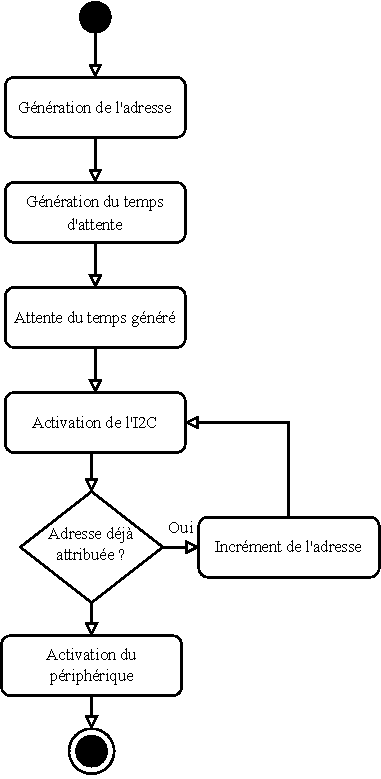
\includegraphics[scale=1.3]{./assets/figures/gen_addr.pdf}
    \caption{Algorithme de génération d'adresse I2C}
\end{figure}

\section{CI/CD}

L'intégration continue (CI) et le déploiement continu (CD) sont deux pratiques utilisées dans le développement de logiciels pour améliorer la qualité, la rapidité et l'efficacité du processus de développement.

\subsection{Définitions}

L'intégration continue consiste à fusionner régulièrement le code développé par les différents membres d'une équipe dans un référentiel central.
Cela permet de détecter rapidement les éventuels problèmes d'incompatibilité ou d'erreur de code, car chaque modification est automatiquement testée et intégrée au code existant.
Les développeurs reçoivent ainsi rapidement des informations sur la validité de leurs modifications, ce qui permet de corriger les erreurs plus tôt dans le processus de développement.

Le déploiement continu, quant à lui, va plus loin en automatisant la phase de déploiement du logiciel.
Une fois que le code a été intégré et testé avec succès, le processus de déploiement se déclenche automatiquement, permettant ainsi la mise à disposition rapide du logiciel aux utilisateurs finaux.
Cela peut inclure le déploiement sur des serveurs de production, la mise à jour des applications ou même la publication sur des plateformes d'applications.

En combinant l'intégration continue et le déploiement continu, les équipes de développement peuvent assurer une livraison plus fréquente et plus fiable des fonctionnalités du logiciel.
Les tests automatisés et l'automatisation du déploiement réduisent les risques d'erreurs, de conflits de code et de problèmes de déploiement, tout en accélérant le cycle de développement global.
Cela permet aux équipes de fournir plus rapidement de nouvelles fonctionnalités et de répondre aux besoins changeants des utilisateurs de manière plus efficace.

\subsection{Objectifs}

Au sein du projet, l'utilisation de l'intégration continue et du déploiement continu est considérée comme une approche pertinente.
L'objectif est d'automatiser la mise à jour du micrologiciel embarqué des périphériques concernés au sein de l'écosystème en cas de modifications apportées à la base de code.
Lorsqu'une mise à jour est effectuée, le système effectue une vérification de la faisabilité de la construction du micrologiciel, puis procède automatiquement au déploiement sur les périphériques.

\subsection{Fonctionnement}

L'utilisation de GitHub pour mettre en place le système de CI/CD est pertinente en raison de sa vaste communauté et des nombreux paquets disponibles pour automatiser diverses tâches.
Le processus comporte deux étapes principales.

Dans un premier temps, l'objectif est de compiler le code afin de générer le fichier binaire du micrologiciel, qui pourra ensuite être téléversé sur un microcontrôleur.

Dans un deuxième temps, il est souhaitable de téléverser le micrologiciel sur les microcontrôleurs concernés, si cela est possible.
Cette étape nécessite une attention particulière, car le maître I2C doit être connecté à Internet.
Si tel est le cas, il peut recevoir une notification indiquant la disponibilité d'une nouvelle version du micrologiciel et procéder à sa mise à jour directement sur les microcontrôleurs. Dans le cas où le maître I2C ne dispose pas d'une connexion Internet, la mise à jour sera effectuée dès que le maître I2C sera allumé et connecté à Internet.

En résumé, le système présenté offre la possibilité de mettre à jour les composants du bus I2C de manière automatique en modifiant le code sur Github à partir de n'importe quel ordinateur.
Cette approche présente un avantage significatif en termes de flexibilité, évitant ainsi les contraintes liées à une mise à jour traditionnelle qui exige l'utilisation d'un câble de reprogrammation pour chaque périphérique.

\section{Gestion des erreurs}

La gestion des erreurs n'étant pas prise en charge de manière native sur un bus I2C, il est pertinent de mettre en place un système de secours pour redémarrer les périphériques en cas de problèmes.
Dans un premier temps, il est nécessaire de détecter les erreurs.
Cette tâche peut être complexe à première vue, car les erreurs doivent être détectées depuis les périphériques esclaves du bus, étant donné que c'est l'élément contrôlé de manière totale.

Dans un deuxième temps, il est requis de trouver une solution pour résoudre le problème.
La solution la plus simple consiste à redémarrer le microcontrôleur.
Cela garantit que si le maître I2C bloque la communication sur le périphérique, le redémarrage mettra fin à cet échange et réglera le problème.

Afin d'explorer les différentes solutions possibles pour détecter les erreurs de manière efficace, cette section se concentrera sur cette problématique.

\subsection{Passage en mode maître}

Une solution envisagée pour détecter les erreurs sur le bus I2C consiste à transformer périodiquement les esclaves I2C en maîtres pour analyser le bus.
Cela permettrait de détecter facilement les erreurs sur le bus.
Cependant, cette approche présente un désavantage important : lorsque le périphérique est en mode maître, il n'est plus disponible en tant qu'esclave pour répondre à ses tâches habituelles.

Ce désavantage rend cette solution non viable, car il est inacceptable de rendre le système inopérant pour détecter les erreurs du bus.

\subsection{Analyse des signaux}

L'analyse des signaux est une solution qui consiste à determiner ce qui est acceptable sur les signaux de l'I2C soit SDA et SCL. Une fois le comportement determiné, il est possible de determiner un comportement qui pose problème. En tant qu'esclave du bus I2C, il est possible d'analyser les signaux du bus I2C sans mettre en péril les communications I2C courantes.